% SYLLABUS ----
% This is just here so I know exactly what I'm looking at in Rstudio when messing with stuff.
\documentclass[11pt,]{article}
\usepackage[margin=1in]{geometry}
\newcommand*{\authorfont}{\fontfamily{phv}\selectfont}
\usepackage[]{mathpazo}
\usepackage{abstract}
\renewcommand{\abstractname}{}    % clear the title
\renewcommand{\absnamepos}{empty} % originally center
\newcommand{\blankline}{\quad\pagebreak[2]}

\providecommand{\tightlist}{%
  \setlength{\itemsep}{0pt}\setlength{\parskip}{0pt}}
\usepackage{longtable,booktabs}

\usepackage{parskip}
\usepackage{titlesec}
\titlespacing\section{0pt}{12pt plus 4pt minus 2pt}{6pt plus 2pt minus 2pt}
\titlespacing\subsection{0pt}{12pt plus 4pt minus 2pt}{6pt plus 2pt minus 2pt}

\titleformat*{\subsubsection}{\normalsize\itshape}

\usepackage{titling}
\setlength{\droptitle}{-.25cm}

%\setlength{\parindent}{0pt}
%\setlength{\parskip}{6pt plus 2pt minus 1pt}
%\setlength{\emergencystretch}{3em}  % prevent overfull lines

\usepackage[T1]{fontenc}
\usepackage[utf8]{inputenc}

\usepackage{fancyhdr}
\pagestyle{fancy}
\usepackage{lastpage}
\renewcommand{\headrulewidth}{0.3pt}
\renewcommand{\footrulewidth}{0.0pt}

\lhead{}
\chead{}
\rhead{\footnotesize EH 0000: A Class with an R Markdown
Syllabus -- Spring 2021}
\lfoot{}
\cfoot{\small \thepage/\pageref*{LastPage}}
\rfoot{}

\fancypagestyle{firststyle}
{
\renewcommand{\headrulewidth}{0pt}%
   \fancyhf{}
   \fancyfoot[C]{\small \thepage/\pageref*{LastPage}}
}

%\def\labelitemi{--}
%\usepackage{enumitem}
%\setitemize[0]{leftmargin=25pt}
%\setenumerate[0]{leftmargin=25pt}




\makeatletter
\@ifpackageloaded{hyperref}{}{%
\ifxetex
  \usepackage[setpagesize=false, % page size defined by xetex
              unicode=false, % unicode breaks when used with xetex
              xetex]{hyperref}
\else
  \usepackage[unicode=true]{hyperref}
\fi
}
\@ifpackageloaded{color}{
    \PassOptionsToPackage{usenames,dvipsnames}{color}
}{%
    \usepackage[usenames,dvipsnames]{color}
}
\makeatother
\hypersetup{breaklinks=true,
            bookmarks=true,
            pdfauthor={ ()},
             pdfkeywords = {},
            pdftitle={EH 0000: A Class with an R Markdown Syllabus},
            colorlinks=true,
            citecolor=blue,
            urlcolor=blue,
            linkcolor=magenta,
            pdfborder={0 0 0}}
\urlstyle{same}  % don't use monospace font for urls


\setcounter{secnumdepth}{0}


\usepackage{graphicx}
% We will generate all images so they have a width \maxwidth. This means
% that they will get their normal width if they fit onto the page, but
% are scaled down if they would overflow the margins.
\makeatletter
\def\maxwidth{\ifdim\Gin@nat@width>\linewidth\linewidth
\else\Gin@nat@width\fi}
\makeatother
\let\Oldincludegraphics\includegraphics
\renewcommand{\includegraphics}[1]{\Oldincludegraphics[width=\maxwidth]{#1}}



\usepackage{setspace}

\title{EH 0000: A Class with an R Markdown Syllabus}
\author{Steven V. Miller}
\date{Spring 2021}

\usepackage{tikz}

\newcommand{\shrug}[1][]{%
\begin{tikzpicture}[baseline,x=0.8\ht\strutbox,y=0.8\ht\strutbox,line width=0.125ex,#1]
\def\arm{(-2.5,0.95) to (-2,0.95) (-1.9,1) to (-1.5,0) (-1.35,0) to (-0.8,0)};
\draw \arm;
\draw[xscale=-1] \arm;
\def\headpart{(0.6,0) arc[start angle=-40, end angle=40,x radius=0.6,y radius=0.8]};
\draw \headpart;
\draw[xscale=-1] \headpart;
\def\eye{(-0.075,0.15) .. controls (0.02,0) .. (0.075,-0.15)};
\draw[shift={(-0.3,0.8)}] \eye;
\draw[shift={(0,0.85)}] \eye;
% draw mouth
\draw (-0.1,0.2) to [out=15,in=-100] (0.4,0.95);
\end{tikzpicture}}

\newcommand{\pandocbounded}[1]{#1}

\usepackage{float}
\usepackage{graphicx}

\begin{document}

		\maketitle


		\thispagestyle{firststyle}

%	\thispagestyle{empty}


	\noindent \begin{tabular*}{\textwidth}{ @{\extracolsep{\fill}} lr @{\extracolsep{\fill}}}


E-mail: \texttt{\href{mailto:steven.miller@ekohist.su.se}{\nolinkurl{steven.miller@ekohist.su.se}}} & Web: \href{http://svmiller.com/teaching}{\tt svmiller.com/teaching}\\
Office Hours: \shrug  &  Class Hours: \shrug\\
Office: \shrug  & Class Room: \shrug\\
	&  \\

	\hline
	\end{tabular*}

\vspace{2mm}


\section{Course Description}\label{course-description}

You'll learn stuff in this class, I hope. Lorem ipsum dolor sit amet,
consectetur adipiscing elit. Maecenas scelerisque elit sapien, eu
consequat dui blandit in. Vestibulum dignissim feugiat mauris, at
pretium turpis blandit nec. Aliquam porta scelerisque tortor, eget
imperdiet quam dapibus et. Sed ut sollicitudin orci, id elementum arcu.
Sed arcu quam, vestibulum molestie mattis sed, ultricies sed est.
Phasellus eu nunc et urna volutpat pharetra. Donec interdum ante vitae
odio malesuada blandit. Fusce at condimentum libero, eu elementum arcu.
Aenean posuere id lorem in varius. Sed bibendum neque pretium dolor
faucibus, in cursus ipsum suscipit. Lorem ipsum dolor sit amet,
consectetur adipiscing elit. Aliquam erat volutpat. Phasellus mollis
egestas risus, non maximus nisl euismod sit amet. Vestibulum laoreet et
urna vitae rutrum. Donec quis dui elit.

\section{Course Objectives}\label{course-objectives}

\begin{enumerate}
\def\labelenumi{\arabic{enumi}.}
\item
  You'll learn this
\item
  And also that
\item
  Perhaps some of this too.
\end{enumerate}

\section{Required Readings}\label{required-readings}

\section{Course Policy}\label{course-policy}

I will detail the policy for this course below. Basically, don't cheat
and try to learn stuff. Don't be that guy.

\subsection{Grading Policy}\label{grading-policy}

\begin{itemize}
\item
  \textbf{20\%} of your grade will be determined by a midterm during
  normal class hours.
\item
  \textbf{20\%} of your grade will be determined by a term paper that
  documents your appreciation of Foghat's ``Slow Ride'', the most
  important song ever written. ``Slow Ride'' is what Mozart wishes
  \emph{Don Giovanni} could have been.
\item
  \textbf{10\%} of your grade will be determined by your attendance and
  participation in class. Generally, ask questions and answer them.
\item
  \textbf{20\%} of your grade will be determined by a 20-page term paper
  on when exactly ``The Love Boat'' jumped the proverbial shark. You
  will address whether this shark-jumping can be attributed to Ted
  McGinley, the introduction of Jill Whelan as ``Vicki'', or some other
  cause.
\item
  \textbf{30\%} of your grade will be determined by a final exam.
\end{itemize}

\subsection{Attendance Policy}\label{attendance-policy}

\begin{quote}
\emph{Showing up is 80 percent of life} -- Woody Allen,
\href{http://quoteinvestigator.com/2013/06/10/showing-up/\#note-6553-1}{via
Marshall Brickman}
\end{quote}

Students should be weary of skipping class. I deduct \emph{all}
participation points for a class after five unexcused absences and this
can have important implications for a student's overall grade in the
class. There is already a strong positive correlation between the
percentage of classes a student has attended in the course and the
student's final grade for the semester (\emph{r} = 0.662) for all 800
students I have taught since Fall 2014.

A simple linear regression of a student's final grade on percentage of
classes attended for the semester for all classes I have taught since
Fall 2014 suggests an increase of one percent in attendance for the
semester leads to an estimated increase of 0.711 in the student's final
grade. Whereas one missed classes constitutes about a five-percent
decrease in percentage attendance for the semester, one missed class
means an estimated decrease of 3.555 in the overall grade. The effect of
attendance on the final grade for the class is precise (\emph{t} =
24.926) and the likelihood that there is no actual relationship between
attendance and final grade for the semester is almost zero. This simple
linear model with just one predictor (attendance) provides a good fit as
well (R\(^2\) = 0.438). See Figure 1 in this document.

\begin{figure}
\centering
\pandocbounded{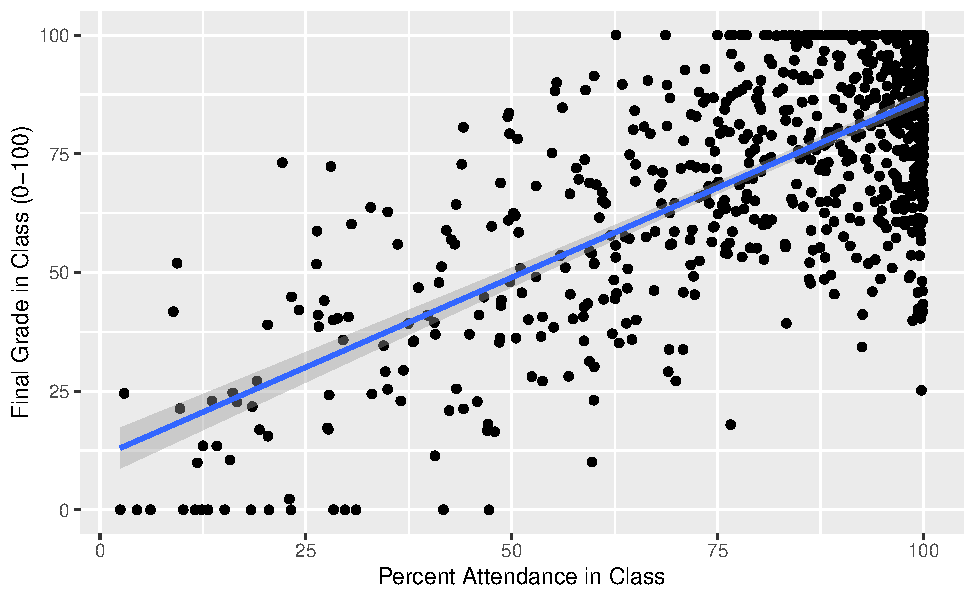
\includegraphics[keepaspectratio]{figs/attendplot.pdf}}
\caption{A Scatterplot of the Relationship between Class Attendance and
Final Grade}
\end{figure}

A student might object that attendance is partly endogenous to a grade
since past classes deducted all participation points after five
unexcused absences. This is true, but the findings hold even when I
subset the data to cases where attendance is greater than 75\%
(i.e.~roughly the threshold below which I deduct all participation
points). Students who just meet the threshold for full participation
points nevertheless get an estimated decrease of 3.375 in their overall
grade for each missed class. This effect is also precise (\emph{t} =
6.664). Put another way, we would have observed this effect in my data
if there were no \emph{true} effect of attendance on grades about 0
times in 100,000 ``trials'' (i.e.~\emph{p} = 0), on average. That
probability is effectively zero. \emph{Attend class}.

\subsection{Late Arrival of the Professor
Policy}\label{late-arrival-of-the-professor-policy}

My current university, from what I have been told, asks professors to
have policies written into their syllabus about what students should do
if the professor is more than 15 minutes late to class. This seems like
an anachronism. I will inform students via e-mail in advance of class if
class is cancelled for the day. I will also contact our department
secretary if something happened on the way to work. Failing that, assume
the worst happened to me. I ask the students make sure that my story
gets the proper treatment on an \emph{Investigation Discovery} show. I
also ask that my story be narrated by Keith Morrison.

\subsection{E-mail Policy}\label{e-mail-policy}

I am usually quick to respond to student e-mails. However, student
e-mails tend to do several things that try my patience. I have a new
policy, effective Fall 2016, that outlines why I will not respond to
certain e-mails students send. Multiple rationales follow.

\begin{enumerate}
\def\labelenumi{\arabic{enumi}.}
\tightlist
\item
  The student could answer his/her own inquiry by reading the syllabus.
\item
  The student missed class for which there was no exam. I do not need to
  know the exact reason for a missed class. Students with excusable
  absences are responsible for giving me a note \emph{in hard copy} that
  documents the reason for the missed class. An e-mail is unnecessary
  unless the impromptu absence involved missing a midterm or final.
\item
  The student wants to know what topics s/he missed during a class s/he
  skipped. The answer is always ``you missed what was on the syllabus.''
\item
  The student is protesting a grade without reference to specific points
  of objection. See the policy on protesting a grade in the syllabus.
  These e-mails tend to be expressive utility on the part of the student
  and do not require a response from me. Students interested in
  improving their knowledge of material should see me during office
  hours.
\item
  The students wants to know how many classes s/he missed at some point
  during the semester. I assume the student has a better answer to that
  question than me until the end of the semester.
\item
  The student is requesting an extension on an assignment for which the
  syllabus already established the deadline. The answer is always
  ``no''.
\item
  The student is
  \href{https://www.math.uh.edu/~tomforde/GradeGrubbing.html}{``grade
  grubbing''} or asking to round up a grade. The answer is always
  ``no''.
\item
  The student is asking for an extra credit opportunity, a request that
  amounts to more grading for the professor. The answer is ``no''.
\end{enumerate}

\subsection{Make-Up Exam Policy}\label{make-up-exam-policy}

There are \textbf{NO} make-ups for missed exams. Don't bother asking.

\subsection{Academic Dishonesty
Policy}\label{academic-dishonesty-policy}

Don't cheat. Don't be that guy. Yes, you. You know exactly what I'm
talking about too.

\subsection{Disabilities Policy}\label{disabilities-policy}

Federal law mandates the provision of services at the university-level
to qualified students with disabilities. Make sure to include all that
relevant information here.

\newpage

\section{Class Schedule}\label{class-schedule}

Students must read the following before Tuesday's class session.
Important: class readings are subject to change, contingent on
mitigating circumstances and the progress we make as a class. Students
are encouraged to attend lectures and check the course website for
updates.

Here is that calendar I promised.

\begin{figure}
\centering
\pandocbounded{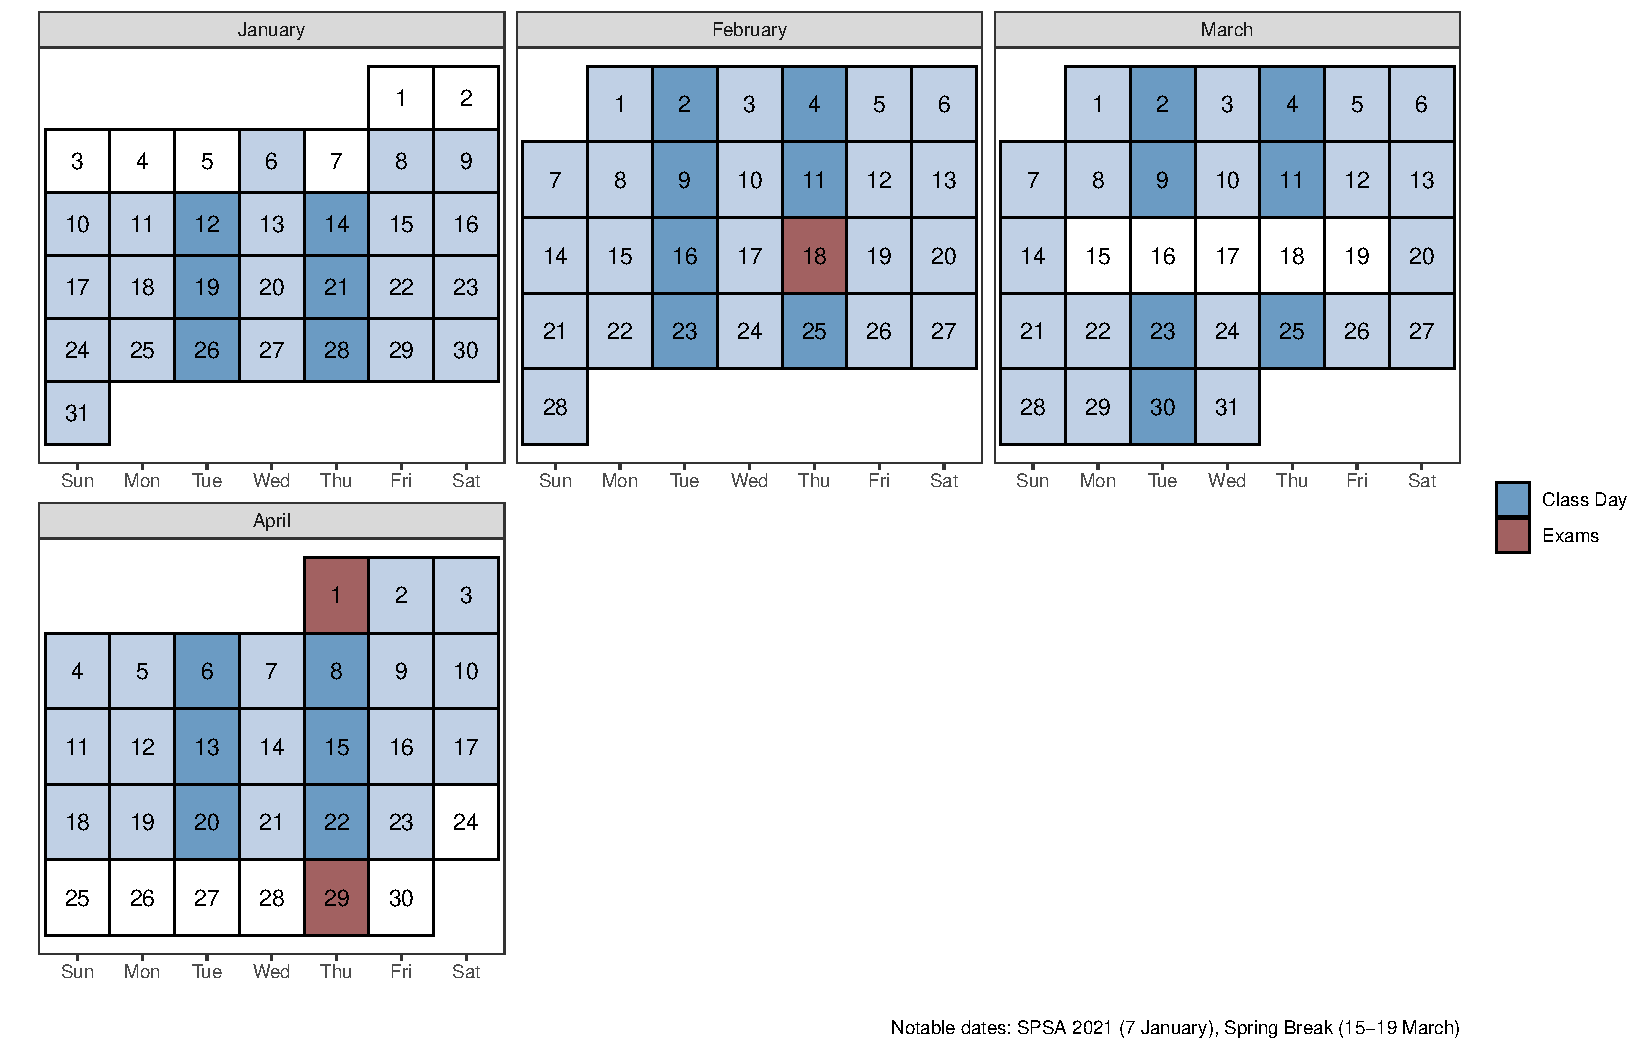
\includegraphics[keepaspectratio]{figs/calendar.pdf}}
\caption{A Calendar for the Class (My Class Title, Spring 2021)}
\end{figure}

\subsection{Week 01, 01/04 - 01/08: Syllabus
Day}\label{week-01-0104---0108-syllabus-day}

\emph{No class Thursday (Political scientists usually have a conference
to start the semester).}

Read \emph{all} associated documents on course website.

\begin{itemize}
\tightlist
\item
  \href{http://svmiller.com/blog/2014/09/taking-good-notes/}{Taking Good
  Notes}
\item
  \href{http://svmiller.com/blog/2015/06/dos-and-donts-of-writing-for-students/}{Dos
  and Dont's of Writing for Students}
\item
  \href{http://svmiller.com/blog/2015/12/assorted-tips-students-research-papers/}{Assorted
  Tips for Students on Writing Research Papers}
\item
  \href{https://www.dropbox.com/s/apihjs7di81aqcv/svm-exam-grading-policy.pdf?dl=0}{Exam
  Grading Policy}
\item
  \href{http://svmiller.com/blog/2016/05/fun-with-attendance-grades/}{Fun
  with Attendance and Grades (i.e.~Students Should Attend Class)}
\end{itemize}

\subsection{Week 02, 01/11 - 01/15: The First
Topic}\label{week-02-0111---0115-the-first-topic}

fdsfsf

\subsection{Week 03, 01/18 - 01/22: The Second
Topic}\label{week-03-0118---0122-the-second-topic}

\emph{Your ``Slow Ride'' appreciation paper is due in Thursday's class}.

\subsection{Week 04, 01/25 - 01/29: Another
Topic}\label{week-04-0125---0129-another-topic}

\subsection{Week 05, 02/01 - 02/05: The Fourth
Topic}\label{week-05-0201---0205-the-fourth-topic}

\subsection{Week 06, 02/08 - 02/12:
Keep}\label{week-06-0208---0212-keep}

\subsection{Week 07, 02/15 - 02/19:
Going}\label{week-07-0215---0219-going}

\subsection{Week 08, 02/22 - 02/26:
Down}\label{week-08-0222---0226-down}

\subsection{Week 09, 03/01 - 03/05: the}\label{week-09-0301---0305-the}

\subsection{Week 10, 03/08 - 03/12:
Line}\label{week-10-0308---0312-line}

\subsection{Week 11, 03/15 - 03/19:
Until}\label{week-11-0315---0319-until}

\subsection{Week 12, 03/22 - 03/26: You}\label{week-12-0322---0326-you}

\subsection{Week 13, 03/29 - 04/02: Are}\label{week-13-0329---0402-are}

\subsection{Week 14, 04/05 - 04/09:
Done}\label{week-14-0405---0409-done}

\subsection{Week 15, 04/12 - 04/16:
with}\label{week-15-0412---0416-with}

\subsection{Week 16, 04/19 - 04/23:
your}\label{week-16-0419---0423-your}

\subsection{Week 17, 04/26 - 04/30:
Syllabus}\label{week-17-0426---0430-syllabus}




\end{document}

\makeatletter
\def\@maketitle{%
  \newpage
%  \null
%  \vskip 2em%
%  \begin{center}%
  \let \footnote \thanks
    {\fontsize{18}{20}\selectfont\raggedright  \setlength{\parindent}{0pt} \@title \par}%
}
%\fi
\makeatother
